\documentclass[11pt,a4paper]{article}
\usepackage[utf8]{inputenc}
\usepackage[french]{babel}
\usepackage[T1]{fontenc}

\usepackage{amsmath}
\usepackage{amsfonts}
\usepackage{amssymb}

\newcommand{\NomAuteur}{Fabrice BOISSIER}
\newcommand{\TitreMatiere}{Algo et Structure de Données 2}
\newcommand{\NomUniv}{EPITA - Bachelor Cyber Sécurité}
\newcommand{\NiveauUniv}{CYBER1}
\newcommand{\NumGroupe}{CYBER1}
\newcommand{\AnneeUniv}{2022-2023}
\newcommand{\DateExam}{Mars 2023}
\newcommand{\TypeExam}{QCM 1}
\newcommand{\TitreExam}{\TitreMatiere}
\newcommand{\DureeExam}{20 min}
\newcommand{\MyWaterMark}{\AnneeUniv} % Watermark de protection

% Ajout de mes classes & definitions
\usepackage{MetalExam} % Appelle un .sty

% "Tableau" et pas "Table"
\addto\captionsfrench{\def\tablename{Tableau}}

%%%%%%%%%%%%%%%%%%%%%%%
%Header
%%%%%%%%%%%%%%%%%%%%%%%
\lhead{\TypeExam}							%Gauche Haut
\chead{\NomUniv}							%Centre Haut
\rhead{\NumGroupe}							%Droite Haut
\lfoot{\DateExam}							%Gauche Bas
\cfoot{\thepage{} / \pageref*{LastPage}}	%Centre Bas
\rfoot{\texttt{\TitreMatiere}}				%Droite Bas

%%%%%

\usepackage{tabularx}

\newlength{\LabelWidth}%
%\setlength{\LabelWidth}{1.3in}%
\setlength{\LabelWidth}{1cm}%
%\settowidth{\LabelWidth}{Employee E-mail:}%  Specify the widest text here.

% Optional first parameter here specifies the alignment of
% the text within the \makebox.  Default is [l] for left
% alignment. Other options are [r] and [c] for right and center
\newcommand*{\AdjustSize}[2][l]{\makebox[\LabelWidth][#1]{#2}}%


\definecolor{mGreen}{rgb}{0,0.6,0}
\definecolor{mGray}{rgb}{0.5,0.5,0.5}
\definecolor{mPurple}{rgb}{0.58,0,0.82}
\definecolor{backgroundColour}{rgb}{0.95,0.95,0.92}

\lstdefinestyle{CStyle}{
    backgroundcolor=\color{backgroundColour},
    commentstyle=\color{mGreen},
    keywordstyle=\color{magenta},
    numberstyle=\tiny\color{mGray},
    stringstyle=\color{mPurple},
    basicstyle=\footnotesize,
    breakatwhitespace=false,
    breaklines=true,
    captionpos=b,
    keepspaces=true,
    numbers=left,
    numbersep=5pt,
    showspaces=false,
    showstringspaces=false,
    showtabs=false,
    tabsize=2,
    language=C
}


\hyphenation{op-tical net-works SIGKILL}


\begin{document}

% \MakeExamTitleDuree     % Pour afficher la duree
\MakeExamTitle                   % Ne pas afficher la duree

%% \MakeStudentName    %% A reutiliser sur chaque nouvelle page


% \setcounter{section}{1}  % Ne pas faire une liste de 0.1, 0.2, ... mais 1.1, 1.2, ...

\renewcommand{\thesubsection}{\arabic{subsection}} % Subsection sans 0.x, mais juste x

% \newcommand{\thesubsection}{\thesection.\arabic{subsection}} % Subsection avec numero section (0.x)


\vfillFirst

\subsection{(4 points) Cochez l'arité/le degré de l'arbre suivant : }

\begin{table}[ht!]
  \centering
  \begin{minipage}{0.30\textwidth}
    \centering

\begin{itemize}
  \item[\CaseCoche] 0 \phantom{()} \\
  \item[\CaseCoche] 1 \phantom{()} \\
  \item[\CaseCoche] 2 \phantom{()} \\
  \item[\CaseCoche] 3 \phantom{()} \\ %
  \item[\CaseCoche] 4 \phantom{()} \\
  \item[\CaseCoche] 14 \phantom{()} \\
\end{itemize}

  \end{minipage}
  \hfillx
  \begin{minipage}{0.60\textwidth}
    \centering

\begin{tikzpicture}[sibling distance=0cm, level distance=12mm,
  leaf/.style = {circle, forestgreen(traditional), draw=green(htmlcssgreen), very thick},
  root/.style = {circle, harvardcrimson, draw=red, very thick},
  internal/.style = {circle, auburn, draw=auburn, very thick},
  level/.style = {sibling distance = 35mm/#1},
  level 3/.style={sibling distance = 8mm},
  every node/.style = {minimum width = 2em, draw, circle},
  ]
  \node {42}
  child { node {21}
          child { node {8}
                  child { node {2} }
                  child { node {16} }
                }
          child { node {24}
                  child { node {22} }
                  child { node {32} }
                }
          child { node {36}
                  child { node {40} }
                }
        }
  child { node {64}
          child { node {96}
                  child { node {72} }
                  child { node {98} }
                }
        };
\end{tikzpicture}

  \end{minipage}
%  \caption{Algorithme de la somme des N premiers entiers}
%  \label{somme-n-premiers-entiers}
\end{table}

\bigskip
%\vspace*{1cm}
\vspace*{0.5cm}

\subsection{(4 points) Cocher les bonnes hauteur et taille de l'arbre suivant : }


\begin{table}[ht!]
  \centering
  \begin{minipage}{0.15\textwidth}
    \centering
Hauteur :

\medskip

\begin{itemize}
  \item[\CaseCoche] 0 \phantom{()} \\
  \item[\CaseCoche] 1 \phantom{()} \\
  \item[\CaseCoche] 2 \phantom{()} \\
  \item[\CaseCoche] 3 \phantom{()} \\ %
  \item[\CaseCoche] 4 \phantom{()} \\
  \item[\CaseCoche] 14 \phantom{()} \\
\end{itemize}

  \end{minipage}
  \hfillx
  \begin{minipage}{0.15\textwidth}
    \centering
Taille :

\medskip

\begin{itemize}
  \item[\CaseCoche] 0 \phantom{()} \\
  \item[\CaseCoche] 1 \phantom{()} \\
  \item[\CaseCoche] 2 \phantom{()} \\
  \item[\CaseCoche] 3 \phantom{()} \\
  \item[\CaseCoche] 4 \phantom{()} \\
  \item[\CaseCoche] 14 \phantom{()} \\ %
\end{itemize}

  \end{minipage}
  \hfillx
  \begin{minipage}{0.60\textwidth}
    \centering

\begin{tikzpicture}[sibling distance=0cm, level distance=12mm,
  leaf/.style = {circle, forestgreen(traditional), draw=green(htmlcssgreen), very thick},
  root/.style = {circle, harvardcrimson, draw=red, very thick},
  internal/.style = {circle, auburn, draw=auburn, very thick},
  level/.style = {sibling distance = 35mm/#1},
  level 3/.style={sibling distance = 8mm},
  every node/.style = {minimum width = 2em, draw, circle},
  ]
  \node {42}
  child { node {21}
          child { node {8}
                  child { node {2} }
                  child { node {16} }
                }
          child { node {24}
                  child { node {22} }
                  child { node {32} }
                }
        }
  child { node {64}
          child { node {48}
                  child [missing] {}
                  child { node {56} }
                }
          child { node {96}
                  child { node {72} }
                  child { node {98} }
                }
        };
\end{tikzpicture}

  \end{minipage}
%  \caption{Algorithme de la somme des N premiers entiers}
%  \label{somme-n-premiers-entiers}
\end{table}


\bigskip
%\vspace*{1cm}
\vspace*{0.5cm}


\subsection{(4 points) Cocher le ou les cas que valident l'arbre suivant : }


\begin{table}[ht!]
  \centering
  \begin{minipage}{0.52\textwidth}
    \centering

\begin{itemize}
  \item[\CaseCoche] Arbre binaire strict / localement complet \phantom{()} \\ %
  \item[\CaseCoche] Arbre binaire parfait \phantom{()} \\
  \item[\CaseCoche] Arbre binaire (presque) complet \phantom{()} \\
  \item[\CaseCoche] Arbre filiforme \phantom{()} \\
  \item[\CaseCoche] Peigne \phantom{()} \\
\end{itemize}

  \end{minipage}
  \hfillx
  \begin{minipage}{0.60\textwidth}
    \centering

\begin{tikzpicture}[sibling distance=0cm, level distance=12mm,
  leaf/.style = {circle, forestgreen(traditional), draw=green(htmlcssgreen), very thick},
  root/.style = {circle, harvardcrimson, draw=red, very thick},
  internal/.style = {circle, auburn, draw=auburn, very thick},
  level/.style = {sibling distance = 35mm/#1},
  level 3/.style={sibling distance = 8mm},
  every node/.style = {minimum width = 2em, draw, circle},
  ]
  \node {42}
  child { node {21}
          child { node {8}
                  child [missing] {}
                  child [missing] {}
                }
          child { node {24}
                  child { node {22} }
                  child { node {32} }
                }
        }
  child { node {64}
          child { node {48}
                  child { node {44} }
                  child { node {56} }
                }
          child { node {96}
                  child { node {72} }
                  child { node {98} }
                }
        };
\end{tikzpicture}

  \end{minipage}
%  \caption{Algorithme de la somme des N premiers entiers}
%  \label{somme-n-premiers-entiers}
\end{table}


\vfillLast

%\bigskip
\newpage

\vfillFirst


\subsection{(4 points) Indiquez le tableau qui représente l'arbre binaire suivant : }

\begin{center}

\begin{tikzpicture}[sibling distance=0cm, level distance=12mm,
  leaf/.style = {circle, forestgreen(traditional), draw=green(htmlcssgreen), very thick},
  root/.style = {circle, harvardcrimson, draw=red, very thick},
  internal/.style = {circle, auburn, draw=auburn, very thick},
  level/.style = {sibling distance = 35mm/#1},
  level 3/.style={sibling distance = 8mm},
  every node/.style = {minimum width = 2em, draw, circle},
  ]
  \node {42}
  child { node {21}
          child { node {8}
                  child [missing] {}
                  child { node {16} }
                }
          child [missing] {}
        }
  child { node {64}
          child { node {48}
                  child [missing] {}
                  child { node {56} }
                }
          child { node {96}
                  child { node {72} }
                  child [missing] {}
                }
        };
\end{tikzpicture}

\end{center}

%\bigskip

\begin{center}
\begin{itemize}
  \item[\CaseCoche] \raisebox{2ex}{
\begin{tabular}{ C{0.5cm} C{0.5cm}C{0.5cm} C{0.5cm}C{0.5cm}C{0.5cm}C{0.5cm} C{0.5cm}C{0.5cm}C{0.5cm}C{0.5cm}C{0.5cm}C{0.5cm}C{0.5cm}C{0.5cm} }
%\begin{tabular}{ c cc cccc cccccccc }
 1 & 2 & 3 & 4 & 5 & 6 & 7 & 8 & 9 & 10 & 11 & 12 & 13 & 14 & 15 \\
\cline{1-15}
\multicolumn{1}{|c|}{42} &
\multicolumn{1}{c|}{21} & \multicolumn{1}{c|}{64} &
\multicolumn{1}{c|}{8} & \multicolumn{1}{c|}{48} &
  \multicolumn{1}{c|}{96} & \multicolumn{1}{c|}{16} &
\multicolumn{1}{c|}{56} & \multicolumn{1}{c|}{72} & \multicolumn{1}{c|}{\footnotesize \textit{-1}} & \multicolumn{1}{c|}{\footnotesize \textit{-1}} &
  \multicolumn{1}{c|}{\footnotesize \textit{-1}} & \multicolumn{1}{c|}{\footnotesize \textit{-1}} & \multicolumn{1}{c|}{\footnotesize \textit{-1}} & \multicolumn{1}{c|}{\footnotesize \textit{-1}} \\
\cline{1-15}
\end{tabular}
}
\\

\bigskip
%\medskip

  \item[\CaseCoche] \raisebox{2ex}{
\begin{tabular}{ C{0.5cm} C{0.5cm}C{0.5cm} C{0.5cm}C{0.5cm}C{0.5cm}C{0.5cm} C{0.5cm}C{0.5cm}C{0.5cm}C{0.5cm}C{0.5cm}C{0.5cm}C{0.5cm}C{0.5cm} }
%\begin{tabular}{ c cc cccc cccccccc }
 1 & 2 & 3 & 4 & 5 & 6 & 7 & 8 & 9 & 10 & 11 & 12 & 13 & 14 & 15 \\
\cline{1-15}
\multicolumn{1}{|c|}{42} &
\multicolumn{1}{c|}{21} & \multicolumn{1}{c|}{8} &
\multicolumn{1}{c|}{\footnotesize \textit{-1}} & \multicolumn{1}{c|}{\footnotesize \textit{-1}} &
  \multicolumn{1}{c|}{16} & \multicolumn{1}{c|}{\footnotesize \textit{-1}} &
\multicolumn{1}{c|}{\footnotesize \textit{-1}} & \multicolumn{1}{c|}{64} & \multicolumn{1}{c|}{48} & \multicolumn{1}{c|}{96} &
  \multicolumn{1}{c|}{\footnotesize \textit{-1}} & \multicolumn{1}{c|}{56} & \multicolumn{1}{c|}{72} & \multicolumn{1}{c|}{\footnotesize \textit{-1}} \\
\cline{1-15}
\end{tabular}
}
\\

\bigskip
%\medskip

  \item[\CaseCoche] \raisebox{2ex}{
\begin{tabular}{ C{0.5cm} C{0.5cm}C{0.5cm} C{0.5cm}C{0.5cm}C{0.5cm}C{0.5cm} C{0.5cm}C{0.5cm}C{0.5cm}C{0.5cm}C{0.5cm}C{0.5cm}C{0.5cm}C{0.5cm} }
%\begin{tabular}{ c cc cccc cccccccc }
 1 & 2 & 3 & 4 & 5 & 6 & 7 & 8 & 9 & 10 & 11 & 12 & 13 & 14 & 15 \\
\cline{1-15}
\multicolumn{1}{|c|}{42} &
\multicolumn{1}{c|}{21} & \multicolumn{1}{c|}{64} &
\multicolumn{1}{c|}{8} & \multicolumn{1}{c|}{\footnotesize \textit{-1}} &
  \multicolumn{1}{c|}{16} & \multicolumn{1}{c|}{\footnotesize \textit{-1}} &
\multicolumn{1}{c|}{48} & \multicolumn{1}{c|}{\footnotesize \textit{-1}} & \multicolumn{1}{c|}{96} & \multicolumn{1}{c|}{\footnotesize \textit{-1}} &
  \multicolumn{1}{c|}{56} & \multicolumn{1}{c|}{\footnotesize \textit{-1}} & \multicolumn{1}{c|}{72} & \multicolumn{1}{c|}{\footnotesize \textit{-1}} \\
\cline{1-15}
\end{tabular}
}
\\

\bigskip
%\medskip

  \item[\CaseCoche] \raisebox{2ex}{
\begin{tabular}{ C{0.5cm} C{0.5cm}C{0.5cm} C{0.5cm}C{0.5cm}C{0.5cm}C{0.5cm} C{0.5cm}C{0.5cm}C{0.5cm}C{0.5cm}C{0.5cm}C{0.5cm}C{0.5cm}C{0.5cm} }
%\begin{tabular}{ c cc cccc cccccccc }
 1 & 2 & 3 & 4 & 5 & 6 & 7 & 8 & 9 & 10 & 11 & 12 & 13 & 14 & 15 \\
\cline{1-15}
\multicolumn{1}{|c|}{42} &
\multicolumn{1}{c|}{21} & \multicolumn{1}{c|}{64} &
\multicolumn{1}{c|}{8} & \multicolumn{1}{c|}{\footnotesize \textit{-1}} &
  \multicolumn{1}{c|}{48} & \multicolumn{1}{c|}{96} &
\multicolumn{1}{c|}{\footnotesize \textit{-1}} & \multicolumn{1}{c|}{16} & \multicolumn{1}{c|}{\footnotesize \textit{-1}} & \multicolumn{1}{c|}{\footnotesize \textit{-1}} &
  \multicolumn{1}{c|}{\footnotesize \textit{-1}} & \multicolumn{1}{c|}{56} & \multicolumn{1}{c|}{72} & \multicolumn{1}{c|}{\footnotesize \textit{-1}} \\
\cline{1-15}
\end{tabular}
}   %%%%%%%%%%%%%%%%%%%
\\
\end{itemize}
\end{center}


%\bigskip
%\vspace*{1cm}
\vspace*{0.5cm}


\subsection{(4 points) Avec un parcours profondeur main gauche en ordre suffixe, dans quel ordre les nœuds seront traités  ? }

\begin{table}[ht!]
  \centering
  \begin{minipage}{0.35\textwidth}
    \centering

\begin{itemize}
  \item[\CaseCoche] A-B-C-D-E-F-G-H-I-J-K \phantom{()} \\
  \item[\CaseCoche] A-B-D-E-H-I-C-F-J-G-K \phantom{()} \\ % Prefixe
  \item[\CaseCoche] A-B-D-H-I-E-J-F-C-K-G \phantom{()} \\
  \item[\CaseCoche] D-B-H-E-I-A-J-F-C-G-K \phantom{()} \\ % Infixe
  \item[\CaseCoche] D-H-I-E-B-J-F-K-G-C-A \phantom{()} \\ % Suffixe
  \item[\CaseCoche] D-H-I-J-E-B-K-F-C-G-A \phantom{()} \\
\end{itemize}

  \end{minipage}
  \hfillx
  \begin{minipage}{0.60\textwidth}
    \centering

\begin{tikzpicture}[sibling distance=0cm, level distance=12mm,
  leaf/.style = {circle, forestgreen(traditional), draw=green(htmlcssgreen), very thick},
  root/.style = {circle, harvardcrimson, draw=red, very thick},
  internal/.style = {circle, auburn, draw=auburn, very thick},
  level/.style = {sibling distance = 35mm/#1},
  level 3/.style={sibling distance = 8mm},
  every node/.style = {minimum width = 2em, draw, circle},
  ]
  \node {A}
  child { node {B}
          child { node {D}
                  child [missing] {}
                  child [missing] {}
                }
          child { node {E}
                  child { node {H} }
                  child { node {I} }
                }
        }
  child { node {C}
          child { node {F}
                  child { node {J} }
                  child [missing] {}
                }
          child { node {G}
                  child [missing] {}
                  child { node {K} }
                }
        };
\end{tikzpicture}

  \end{minipage}
%  \caption{Algorithme de la somme des N premiers entiers}
%  \label{somme-n-premiers-entiers}
\end{table}


%\bigskip
%\vspace*{1cm}
\vspace*{0.5cm}


%\subsection{[BONUS] (0 point) Quel âge semble avoir la femme sur cette image ? }
\subsection{[BONUS] (0 point) De quelle couleur est la robe sur cette image ? }

\centering{
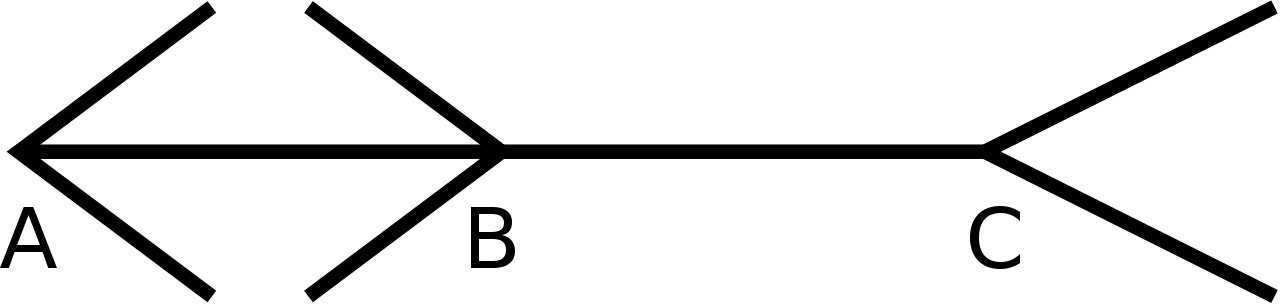
\includegraphics[scale=0.1]{img/illusion de Müller-Lyer ou illusion de Brentano.png}
}

\begin{table}[ht!]
  \centering
  \begin{minipage}{0.40\textwidth}
    \centering
\begin{itemize}
%  \item[\CaseCoche] La robe est bleue et noire \phantom{()} \\
%  \item[\CaseCoche] La robe est blanche et or \phantom{()}\\
  \item[\CaseCoche] C'est une jeune fille \phantom{()} \\
  \item[\CaseCoche] C'est une vieille dame \phantom{()} \\
  \item[\CaseCoche] \raisebox{2ex}{ \rotatebox{180}{42} } \phantom{()} \\
\end{itemize}
  \end{minipage}
  \hfillx
  \begin{minipage}{0.50\textwidth}
    \centering
\begin{itemize}
  \item[\CaseCoche] Ceci n'est pas une absurdité. \phantom{()} \\
  \item[\checkmark] Test. ~ ~ ~ \reflectbox{Pieds.} \phantom{()} \\
  \item[\CaseCoche] \phantom{()} \\
\end{itemize}
  \end{minipage}
%  \caption{Algorithme de la somme des N premiers entiers}
%  \label{somme-n-premiers-entiers}
\end{table}

\vfillLast

\end{document}
